\chapter{満足性とANB及びLLEとの関係性}
\label{chap:pulsewave}

本章では,後述の時系列UX評価システムの開発に先立ち,容積脈波によるストレス指標と満足性の関連を把握するために行った予備実験について述べる.新たなストレス指標としては自律神経バランス(ANB)と最大リヤプノフ指数(LLE)を検討した.また,従来の指標として心拍数(HR)も合わせて計測した.

\section{実験方法}

実験では,Nielsenのヒューリスティクスに基づいて作成した2つのUIを使ったタスクを被験者に実施してもらい,それぞれを使用している際のANBとLLE,HRを比較した.ヒューリスティクスでBad UIとされているものは多くの場合満足性が低くなると考えられるものの,はユーザビリティ評価に使用するものであり,それがそのまま満足性に直結するとはいえない.そこで自己申告メトリクスを併用し,どちらのUIがより好ましかったかについて回答を求めた.

実験は2020年3月に17歳から74歳までの16名(男性13名,女性3名)を対象に行った.

\subsection{実験マテリアルの開発}

UX評価のマテリアルとして,Nielsenのヒューリスティクスで推奨されているUIと避けるべきとされているUIをそれぞれ便宜上Good UIとBad UIと名付け,サンプルとなるアプリケーションを開発した.今回対象としたヒューリスティクスは``Visibility of system status'’(システムの状態の可視性)\cite{nielsen1990} である.10のヒューリスティクス(表\ref{table:heuristics})のなかでアプリケーションの機能に関係ないものや学習が必要なもの,ユーザの予備知識に関係するものなど今回の実験に適さないものを排除して選択した.

\begin{landscape}
\begin{table}[]
\centering
\begin{tabular}{lll}
\hline
原題                                                      & 邦訳              & 例                       \\ \hline
Visibility of system status                             & システムの状態の可視化     & プログレス表示,選択状態表示          \\
Match between system and the real world                 & システムと実世界の対応     & コンロの操作部とバーナーの配置の一致      \\
User control and freedom                                & ユーザによる制御と自由度    & UndoとRedoのサポート          \\
Consistency and standards                               & 一貫性と標準          & OSメーカーによるガイドラインへの準拠     \\
Error prevention                                        & 誤操作の防止          & 破壊的操作時にキャンセルをデフォルトにすること \\
Recognition rather than recall                          & 思い出さずとも認識できること  & 必要な機能がメニューに並んでいること      \\
Flexibility and efficiency of use                       & フレキシブルで効率的      & ショートカットキー               \\
Aesthetic and minimalist design                         & 美しくミニマムなデザイン    & ほとんど必要とされない情報を表示しないこと   \\
Help users recognize, diagnose, and recover from errors & エラーの認識,診断,回復の支援 & 適切なエラーメッセージの表示          \\
Help and documentation                                  & ヘルプとドキュメント      & ヘルプの充実                  \\ \hline
\end{tabular}
\caption{10 Usability Heuristics for User Interface Design\cite{nngroup}}
\label{table:heuristics}
\end{table}
\end{landscape}

具体的にはプログレス表示があるものをGood UI,無いものをBad UIとした.マテリアルの画面は図\ref{fig:old1}の通りである.画面にはノイズにならないように数字を表示するラベルと数字を変更するボタンのみを配置した.また,右上のスイッチでスタッフがGood UIとBad UIを切り替えられるようにした.アプリケーションの機能はNEXTボタンをタップするとランダムで0-5秒後にランダムな数字の表示が切り替わるだけのシンプルなものである.Good UIではNEXTボタンをタップすると図\ref{fig:old2}のようにプログレスを表示するインジケータが表示され,システムが次の数字を読み込み中であるという状態を表示する.一方でBad UIではNEXTボタンを押してもその時点では何の反応もなく,0-5秒後に数字が切り替わるまで上手くタップできたかどうかがわかりにくくなっている.

\begin{figure}[htbp]
  \begin{minipage}{0.5\hsize}
    \begin{center}
       \fbox{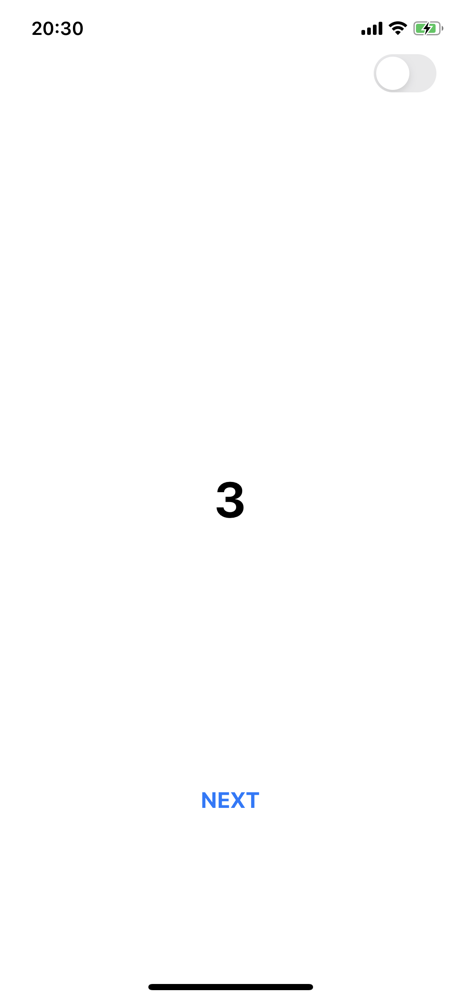
\includegraphics[width=40mm]{img/old1.png}}
    \end{center}
    \caption{実験マテリアル:数字の表示画面}
    \label{fig:old1}
  \end{minipage}
  \begin{minipage}{0.5\hsize}
    \begin{center}
       \fbox{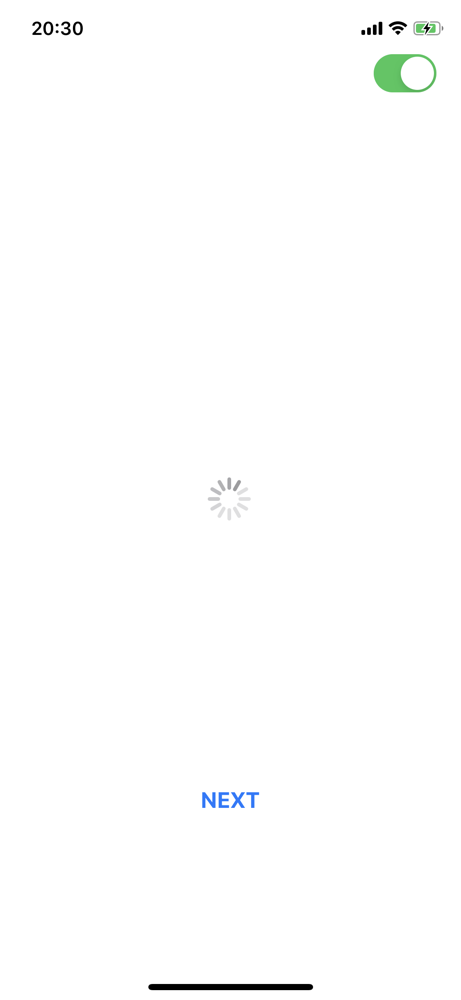
\includegraphics[width=40mm]{img/old2.png}}
    \end{center}
    \caption{実験マテリアル:数字の読込中画面}
    \label{fig:old2}
  \end{minipage}
\end{figure}

\subsection{タスクの実施}
被験者にマテリアルを操作してもらう際には,バイアスがかからないようにダミータスクを用意したうえでGood UIとBad UIそれぞれを順番に実施してもらった.なお,Good UIとBad UIの間には3分間の安静時間を設け,それぞれのマテリアルを操作する順番はカウンターバランスをとった.

ダミータスクは,1分間でNEXTボタンをタップして表示される数字をできるだけ多く書き取るものにした.できるだけ多く書くようにと指示することで,競争意識によって手を抜きにくくなるほか,早く表示してほしいと思わせるように設計した.

\begin{itembox}[l]{タスクの指示}
\begin{verbatim}
今から1分間のテストを2回行ってもらいます.このアプリでは,NEXTボタンを押すと数字が読み込まれますので紙に表示された数字を書いてください.書き終わったらもう一度NEXTボタンを押して次の数字を読み込んで紙に書いてください.制限時間は1分ですのでできるだけ沢山書くようにしてください.ただし,NEXTボタンを押してから数字が読み込まれるまで少し時間がかかりますので待ってください.
\end{verbatim}
\end{itembox}

\subsection{容積脈波(BVP)の計測}
BVPの計測は光学式指尖容積脈波計(PPG)のLifescore Quickプローブ(型番LQ-11,図\ref{fig:device2} )と専用の分析システムであるLyspect\cite{chaotechlyspect}を使用した.Lyspectでは300HzでBVPを記録し,LLEの平均とHF及びLFの値,HRの平均を取得した(図\ref{fig:lyspect}).被験者には実験の開始から終了まで利き手と逆の人差し指にセンサを装着してもらい休憩中も外さないようにした.なお,計測はマテリアルを使用している1分間の間のみとし1人当たり計2回記録した.

\begin{figure}[htbp]
  \begin{minipage}{\hsize}
    \begin{center}
       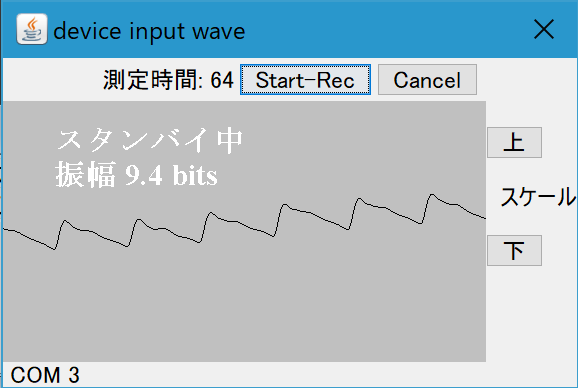
\includegraphics[width=100mm]{img/inputwave}
    \end{center}
    \caption{Lyspectでの計測中画面}
    \label{fig:lyspect}
  \end{minipage}
\end{figure}

\section{結果}

実験の結果を表\ref{table:result1}に示す.カウンターバランスを考慮し,半数の8名はGood  UI - Bad UIの順で実施,残りの被験者には逆の順番で実施した.なお一部の被験者には実験開始直後にセンサのズレを直したことが原因と考えられるBVPの大きな乱れが見られ,その場合にはBVPをトリミングしてLyspectを用いて分析した(図\ref{fig:lyspect_analyze}).

\begin{figure}[htbp]
  \begin{minipage}{\hsize}
    \begin{center}
       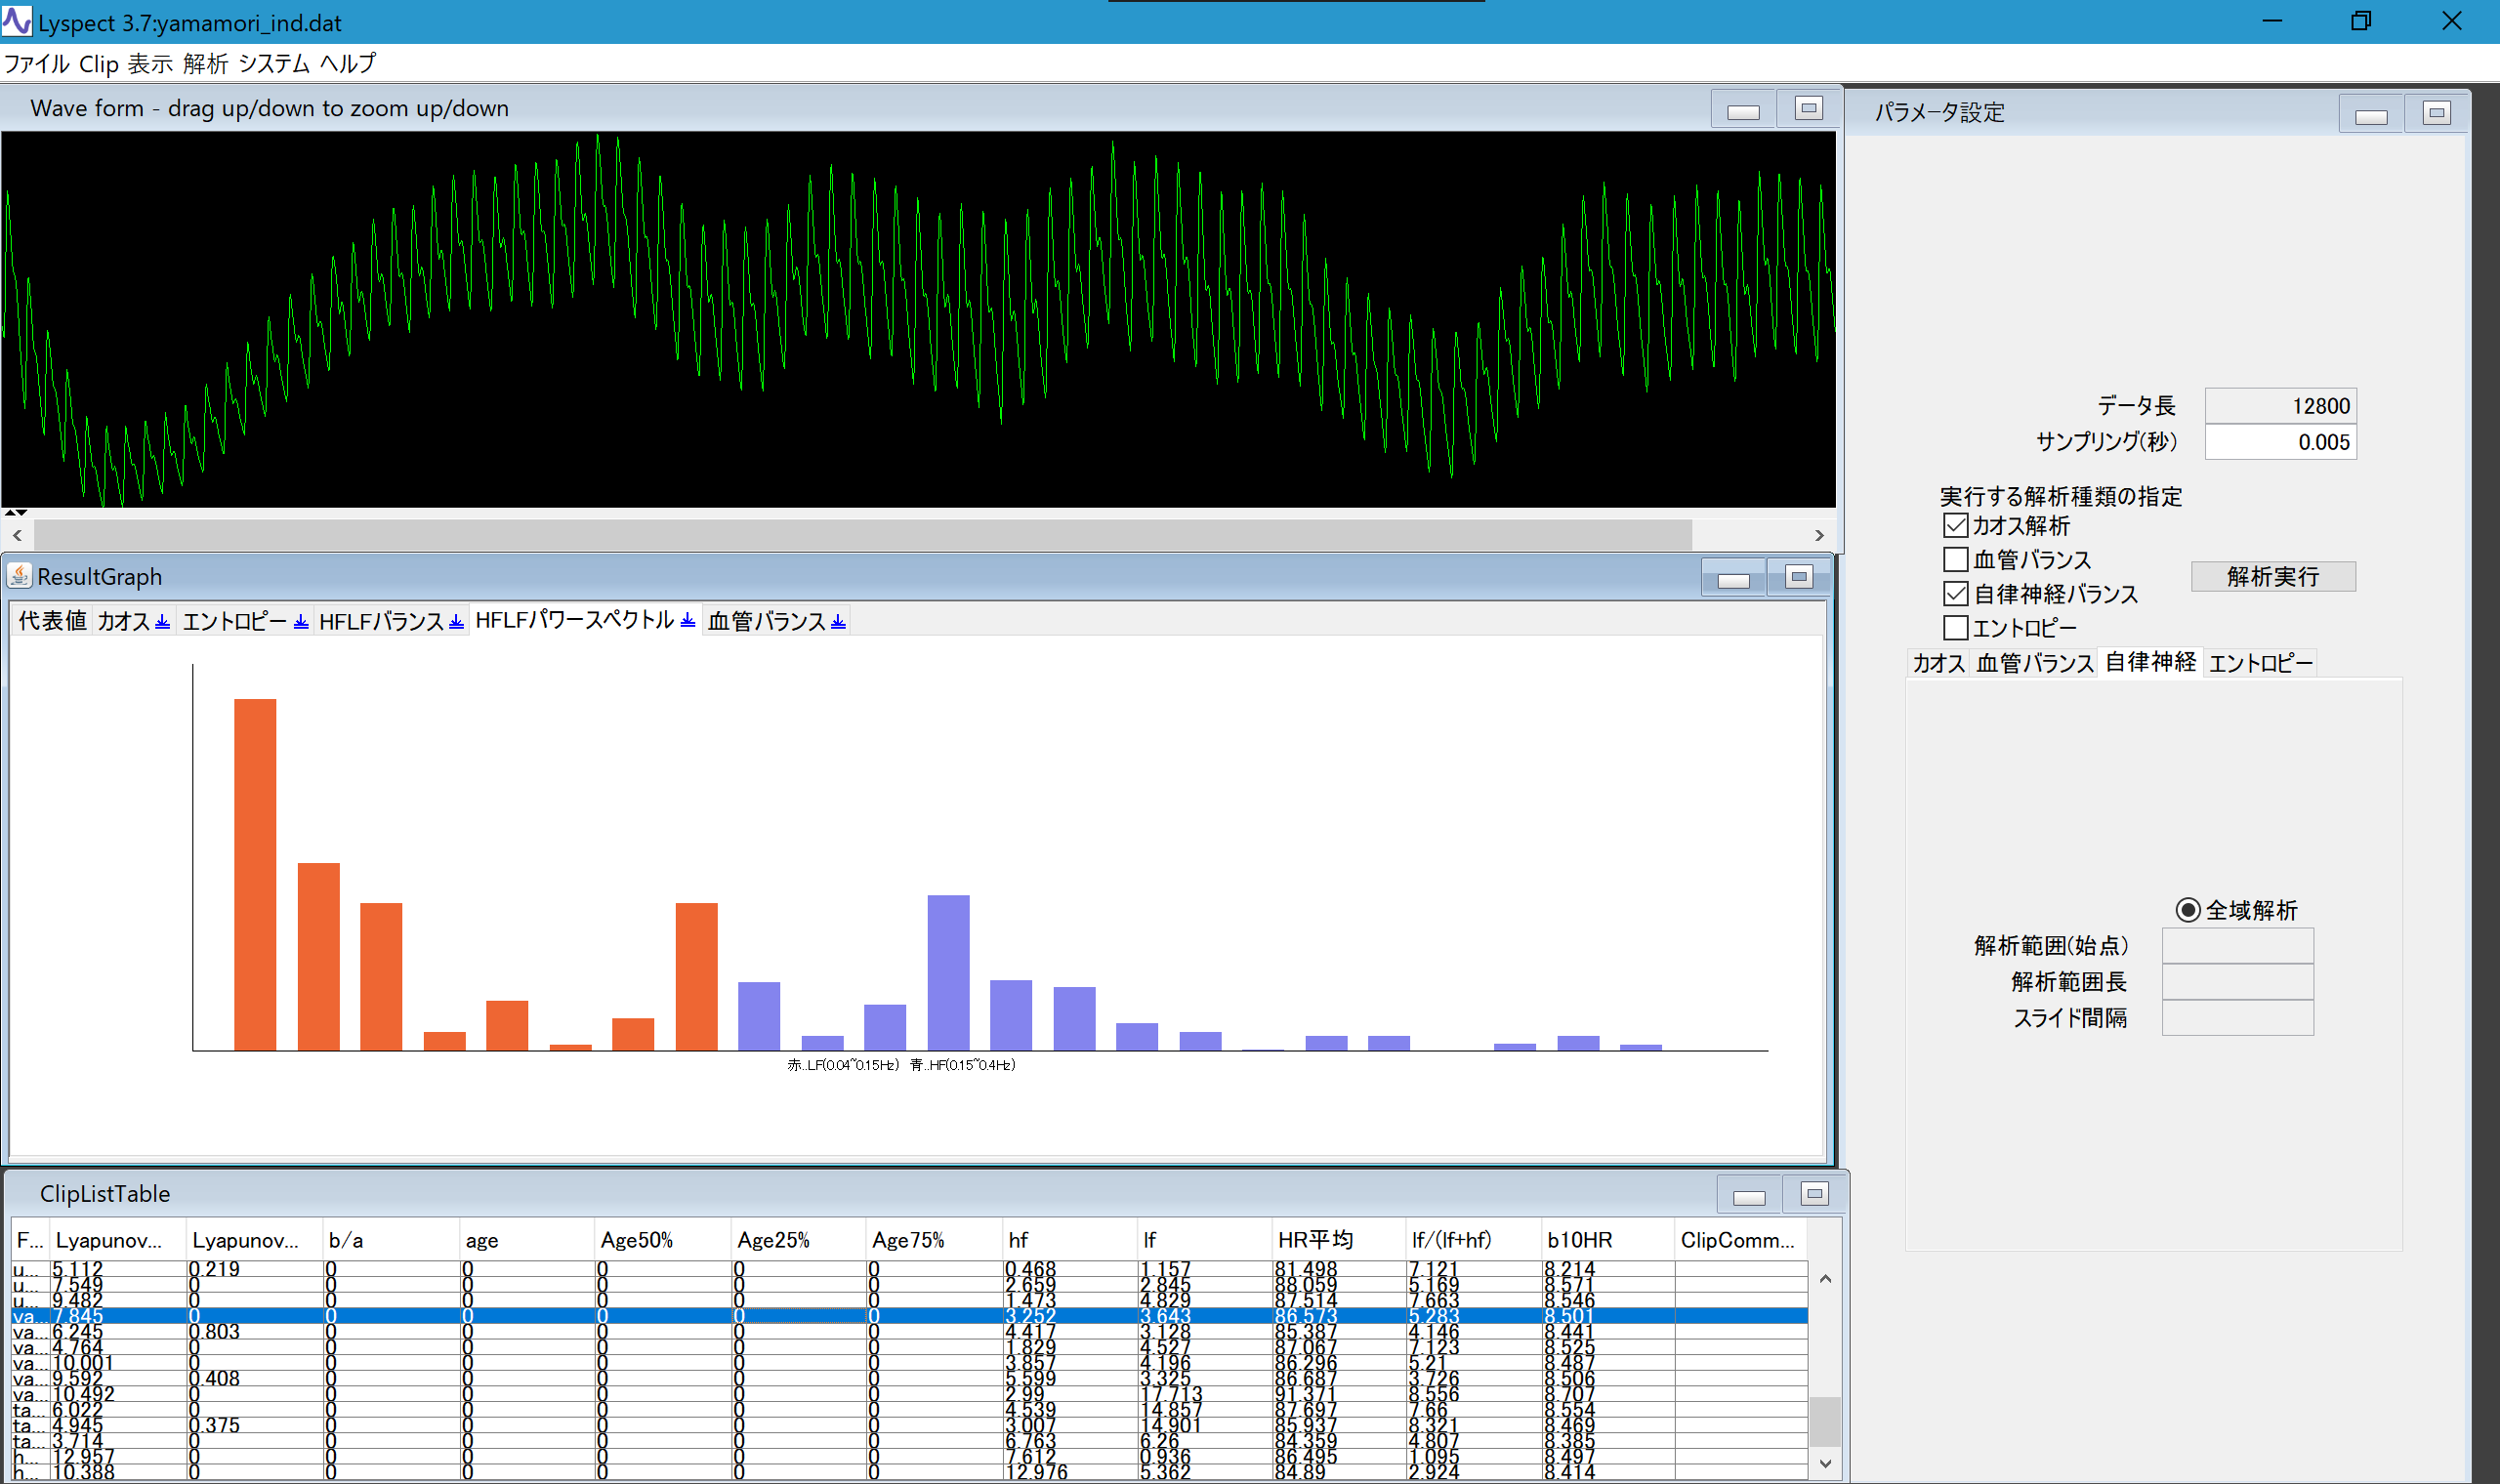
\includegraphics[width=100mm]{img/lyspect_analyze}
    \end{center}
    \caption{Lyspectでの分析画面}
    \label{fig:lyspect_analyze}
  \end{minipage}
\end{figure}

簡単な自己申告メトリクスとして「どちらのUIのほうが使いやすいと感じたか」と質問して得られた結果を表の申告列に表示した.今回ヒューリスティクスに基づいて設定したGood UIは設計としてはユーザビリティが高いと考えられるが,本研究では満足性との関連を調査するため客観的利用品質であるユーザビリティよりも主観的利用品質を優先した.そのため「使いやすいと感じた」と申告されたUIをその被験者にとっての満足性の高いUIとする.

\section{分析}

ANBとLLE,HRを申告に基づいた満足性の高かったUIと低かったUIそれぞれに対応させ,満足性との一致を調べた.前述のようにANBは大きいほうがストレスが高く,LLEはゆらぎの大きさを示し小さい方がストレスが高く,HRは大きい方がストレスが高いと考えられる.これに基づいてANBとLLE,HRそれぞれについて満足性が高かったUIのほうがストレスも低かった場合に一致したとみなした.その結果,表\ref{table:result1-2}のようにANBは16件のうち2件を除いて一致し,LLEは16件中9件しか一致せず,HRは6件しか一致しなかった.

ANB,LLE,HRそれぞれについて満足性の高いUIと満足性の低いUIの値に差が無いかどうか検討するために,満足性を独立変数としANB,LLE,HRをそれぞれ従属変数とした対応のある$t$ 検定を実施した.その結果,ANBでは,満足性の高かったUI($M = 1.84, SD = 1.56$)と満足性の低かったUI($M = 2.91, SD=2.20$)の間でANBに有意な差が見られた($t (15) = -2.14, p=.02, d=.54$).一方,LLEでは,満足性の高かったUI($M = 6.85, SD = 2.63$)と満足性の低かったUI($M = 6.61, SD=2.68$)の間でLLEに有意な差は見られなかった($t (15) = -.67, p=.25, n.s.$).また,HRでも,満足性の高かったUI($M = 79.33, SD = 8.96$)と満足性の低かったUI($M = 78.30, SD = 8.97$)の間でHRに有意な差は見られなかった($t (15) = 1.00, p=.17, n.s.$).

\begin{landscape}
\begin{table}[htbp]
\centering
\begin{tabular}{lllllrrrrrrrrrr}
\hline
\multicolumn{1}{c}{\multirow{2}{*}{No.}} & \multicolumn{1}{c}{\multirow{2}{*}{年齢}} & \multicolumn{1}{c}{\multirow{2}{*}{性別*}} & \multicolumn{1}{c}{\multirow{2}{*}{実験順\dag}} & \multicolumn{1}{c}{\multirow{2}{*}{申告\dag\ddag}} & \multicolumn{5}{l}{Good UI}                                                                                                  & \multicolumn{5}{l}{Bad UI}                                                                                                   \\ \cline{6-15} 
\multicolumn{1}{c}{}                     & \multicolumn{1}{c}{}                    & \multicolumn{1}{c}{}                    & \multicolumn{1}{c}{}                     & \multicolumn{1}{c}{}                    & \multicolumn{1}{c}{HF} & \multicolumn{1}{c}{LF} & \multicolumn{1}{c}{ANB} & \multicolumn{1}{c}{LLE} & \multicolumn{1}{c}{HR} & \multicolumn{1}{c}{HF} & \multicolumn{1}{c}{LF} & \multicolumn{1}{c}{ANB} & \multicolumn{1}{c}{LLE} & \multicolumn{1}{c}{HR} \\ \hline
1                                        & 44                                      & M                                       & G - B                                    & B                                       & 1.30                   & 3.19                   & 2.46                    & 5.26                    & 68.80                  & 2.21                   & 1.87                   & 0.84                    & 6.12                    & 68.10                  \\
2                                        & 18                                      & M                                       & G - B                                    & B                                       & 6.76                   & 6.26                   & 0.93                    & 3.71                    & 88.19                  & 3.01                   & 14.90                  & 4.96                    & 4.95                    & 84.42                  \\
3                                        & 48                                      & F                                       & G - B                                    & G                                       & 1.22                   & 1.13                   & 0.93                    & 3.25                    & 77.177                 & 0.43                   & 1.32                   & 3.09                    & 4.37                    & 82.88                  \\
4                                        & 55                                      & M                                       & G - B                                    & G                                       & 2.39                   & 9.10                   & 3.82                    & 2.74                    & 67.70                  & 1.09                   & 4.33                   & 3.99                    & 2.51                    & 67.39                  \\
5                                        & 26                                      & M                                       & G - B                                    & G                                       & 5.60                   & 3.33                   & 0.93                    & 9.59                    & 86.69                  & 2.99                   & 17.71                  & 5.92                    & 10.49                   & 91.37                  \\
6                                        & 24                                      & M                                       & G - B                                    & G                                       & 18.00                  & 13.38                  & 0.74                    & 9.44                    & 63.23                  & 28.57                  & 9.55                   & 0.33                    & 9.62                    & 64.09                  \\
7                                        & 26                                      & M                                       & G - B                                    & G                                       & 10.10                  & 8.21                   & 0.81                    & 7.49                    & 63.35                  & 6.50                   & 9.04                   & 1.39                    & 6.29                    & 63.69                  \\
8                                        & 19                                      & F                                       & G - B                                    & G                                       & 4.72                   & 3.55                   & 0.75                    & 7.52                    & 79.023                 & 10.42                  & 9.04                   & 0.87                    & 10.43                   & 81.50                  \\
9                                        & 74                                      & F                                       & B - G                                    & G                                       & 1.27                   & 1.49                   & 1.17                    & 5.08                    & 85.39                  & 0.47                   & 1.16                   & 2.47                    & 5.11                    & 87.07                  \\
10                                       & 17                                      & M                                       & B - G                                    & G                                       & 0.91                   & 2.19                   & 2.40                    & 9.50                    & 79.55                  & 1.12                   & 2.88                   & 2.57                    & 7.87                    & 76.40                  \\
11                                       & 24                                      & M                                       & B - G                                    & G                                       & 4.42                   & 3.13                   & 0.71                    & 6.25                    & 87.68                  & 1.83                   & 4.53                   & 2.48                    & 4.76                    & 81.64                  \\
12                                       & 38                                      & M                                       & B - G                                    & G                                       & 2.87                   & 8.41                   & 2.93                    & 4.31                    & 79.79                  & 3.81                   & 12.68                  & 3.33                    & 4.51                    & 69.02                  \\
13                                       & 35                                      & M                                       & B - G                                    & G                                       & 0.61                   & 3.04                   & 4.98                    & 6.05                    & 82.89                  & 0.73                   & 6.55                   & 8.95                    & 5.78                    & 77.78                  \\
14                                       & 20                                      & M                                       & B - G                                    & G                                       & 3.14                   & 7.10                   & 2.26                    & 6.88                    & 84.36                  & 4.46                   & 18.10                  & 4.06                    & 5.17                    & 85.94                  \\
15                                       & 22                                      & M                                       & B - G                                    & G                                       & 7.61                   & 0.94                   & 0.12                    & 12.96                   & 86.50                  & 12.98                  & 5.36                   & 0.41                    & 10.39                   & 84.89                  \\
16                                       & 20                                      & M                                       & B - G                                    & G                                       & 2.66                   & 2.85                   & 1.07                    & 7.55                    & 88.06                  & 1.47                   & 4.83                   & 3.28                    & 9.48                    & 87.51                  \\ \hline
\multicolumn{10}{l}{*Mは男性,Fは女性}\\
\multicolumn{10}{l}{\dag GはGood UI,BはBad UI }\\
\multicolumn{10}{l}{\ddag 申告は聞き取りに対して「使いやすかった」と答えたもの}\\
\end{tabular}
\label{table:result1}
\caption{満足性とANB,LLE,HRとの関係性についての実験結果}
\end{table}
\end{landscape}

\begin{landscape}
\begin{table}[htbp]
\centering
\begin{tabular}{llrrlrrlrrl}
\hline
\multicolumn{1}{c}{No.} & \multicolumn{1}{c}{申告} & \multicolumn{3}{l}{ANB}                                                      & \multicolumn{3}{l}{LLE}                                                      & \multicolumn{3}{l}{HR}                                                       \\ \cline{3-11} 
\multicolumn{1}{c}{}    & \multicolumn{1}{c}{}   & \multicolumn{1}{c}{満足性高} & \multicolumn{1}{c}{満足性低} & \multicolumn{1}{c}{一致} & \multicolumn{1}{c}{満足性高} & \multicolumn{1}{c}{満足性低} & \multicolumn{1}{c}{一致} & \multicolumn{1}{c}{満足性高} & \multicolumn{1}{c}{満足性低} & \multicolumn{1}{c}{一致} \\ \hline
1                       & Bad UI                 & 0.84                     & 2.46                     &                        & 6.12                     & 5.26                     &                        & 68.10                    & 68.80                    & 不一致                    \\
2                       & Bad UI                 & 2.40                     & 2.57                     &                        & 9.50                     & 7.87                     &                        & 88.19                    & 84.42                    & 不一致                    \\
3                       & Good UI                & 0.93                     & 3.09                     &                        & 3.25                     & 4.37                     & 不一致                    & 77.18                    & 82.88                    &                        \\
4                       & Good UI                & 3.82                     & 3.99                     &                        & 2.74                     & 2.51                     &                        & 67.70                    & 67.39                    & 不一致                    \\
5                       & Good UI                & 0.93                     & 5.92                     &                        & 9.59                     & 10.49                    & 不一致                    & 86.69                    & 91.37                    &                        \\
6                       & Good UI                & 0.74                     & 0.33                     & 不一致                    & 9.44                     & 9.62                     & 不一致                    & 63.23                    & 64.09                    &                        \\
7                       & Good UI                & 0.81                     & 1.39                     &                        & 7.49                     & 6.29                     &                        & 63.35                    & 63.69                    &                        \\
8                       & Good UI                & 1.17                     & 2.47                     &                        & 5.08                     & 5.11                     & 不一致                    & 79.02                    & 81.50                    &                        \\
9                       & Good UI                & 0.71                     & 2.48                     &                        & 6.25                     & 4.76                     &                        & 85.39                    & 87.07                    &                        \\
10                      & Good UI                & 2.93                     & 3.33                     &                        & 4.31                     & 4.51                     & 不一致                    & 79.55                    & 76.40                    & 不一致                    \\
11                      & Good UI                & 4.98                     & 8.95                     &                        & 6.05                     & 5.78                     &                        & 87.68                    & 81.64                    & 不一致                    \\
12                      & Good UI                & 2.26                     & 4.06                     &                        & 6.88                     & 5.17                     &                        & 79.79                    & 69.02                    & 不一致                    \\
13                      & Good UI                & 0.75                     & 0.87                     &                        & 7.52                     & 10.43                    & 不一致                    & 82.89                    & 77.78                    & 不一致                    \\
14                      & Good UI                & 4.96                     & 0.93                     & 不一致                    & 4.95                     & 3.71                     &                        & 85.94                    & 84.36                    & 不一致                    \\
15                      & Good UI                & 0.12                     & 0.41                     &                        & 12.96                    & 10.39                    &                        & 86.50                    & 84.89                    & 不一致                    \\
16                      & Good UI                & 1.07                     & 3.28                     &                        & 7.55                     & 9.48                     & 不一致                    & 88.06                    & 87.51                    & 不一致                    \\ \hline
\end{tabular}
\label{table:result1-2}
\caption{ANB,LLE,HRと申告に基づく満足性との関係}
\end{table}
\end{landscape}

\section{考察}

本実験の結果を以下に示す.

\begin{enumerate}
\renewcommand{\labelenumi}{(\arabic{enumi})}
  \item ANBは,被験者の満足性が高かったUIを使用した時と低かったUIを使用した時との間で中程度\cite{cohen}に有意な差が見られ,ほとんどの被験者で満足性が高かったUIの使用時のほうが低くなった.
  \item LLEは,被験者の満足性が高かったUIを使用した時と低かったUIを使用した時との間で有意な差が見られなかった.
  \item HRは,被験者の満足性が高かったUIを使用した時と低かったUIを使用した時との間で有意な差が見られなかった.
\end{enumerate}

(1)について考察する.

ANBはシステム使用時の満足性と関係がありUXを評価するための指標として有用である可能性が示された.ANBが高ければストレスが高いと考えられUXが良くないことを示し,逆に低ければストレスも低くUXが良いと言える.また,一方で,今回の実験では被験者の申告に頼っていることや,明らかにストレスがかかりやすいUIをマテリアルとして採用していること,同じ操作を何度も繰り返させることでその変化が数値に表れやすくしていることなどの制約があった.実用化に向けてより多くの種類のUIの問題をこの指標で捉えられるかどうかを明らかにする必要がある.

(2)(3)について考察する.

今回の実験ではLLE,HRと満足性との間に有意な関係性は見られなかった.さらに,LLEとHRそれぞれ約半数の標本で,被験者が申告した満足性の高いUIとLLE,HRの値が一致していなかったことから,今回の計測方法ではLLEとHRが活用できる可能性が低い.HRを使用したユーザビリティ評価の先行研究\cite{trimmel2003stress}では,計測したい一時的UXのイベント直後にECGによって計測したRRIからHRを算出しているため,今回のよりも短い時間で計測していた可能性がある.そのため,RRIレベルの瞬間的なHRを計測すれば満足性を計測できる可能性がある.LLEについても同様に計測時間を短くしたときの満足性との関係性について検討する必要がある.

また,この実験の結果から,これまで使用されてきたHRは一定の条件下で上手く機能せず,またHRが機能しない場合でもANBが活用できる可能性が示唆された.今回の実験では,1分の間で継続的に操作を行ったにも関わらず,HRの平均値には満足性との関係が見られなかった.このことから,仮に操作後に瞬間的なHRの上昇があったとしても持続しないかノイズが多くなっている可能性がある.操作のタイミングとHRの変化の関係性や変化の持続時間などについて検討する必要がある.一方,今回の実験のように待機時間のストレスを測るなど長時間の代表値を得たい場合にはHRではなくANBが有効になる可能性がある.



